\documentclass[10pt]{beamer}

\usetheme[progressbar=frametitle]{metropolis}
\usepackage{appendixnumberbeamer}

\usepackage{booktabs}
\usepackage[scale=2]{ccicons}

\usepackage{pgfplots}
\usepgfplotslibrary{dateplot}

\usepackage{xspace}
\newcommand{\themename}{\textbf{\textsc{metropolis}}\xspace}

\usepackage{verbatim}
\usepackage[utf8]{inputenc}  
\usepackage{subcaption}

\title{NATS: Non-parametric analysis of time series}
%\subtitle{}
% \date{\today}
\date{}
\author{Eduarda Chagas \\ Alejandro Frery \\ Heitor Ramos \\ Osvaldo Rosso}
\institute{UFMG -- Wisemap \\
eduarda.chagas@dcc.ufmg.br}
\titlegraphic{\hfill
\includegraphics[height=0.5cm]{Figures/ufmg.png}}

\begin{document}

\maketitle

\begin{frame}{Summary}
  \setbeamertemplate{section in toc}[sections numbered]
  \tableofcontents[hideallsubsections]
\end{frame}

\section{NATS}

\begin{frame}[fragile]{Objectives}
    
    \textbf{Main objectives}:
    
    \begin{itemize}
        \item Propose and develop an innovative tool for time series analysis, resulting from recent research proposals related to Information Theory, to facilitate the use of advanced signal processing and analysis techniques.
    \end{itemize}
    
    \textbf{Specific objectives}:
    
    \begin{itemize}
        \item The need to make techniques accessible to unskilled users, and
        \item The need to optimize the development of new techniques.
    \end{itemize}

\end{frame}

\begin{frame}[fragile]{Existing tools - CRAN packages}
    
    \textbf{statcomp}:
            \begin{itemize}
                \item fis
                \item global\underline{ } complexity
                \item hellinger\underline{ }distance
                \item jensen\underline{  }shannon\underline{ }divergence
                \item limit\underline{ }curves
                \item MPR\underline{ }complexity
                \item ordinal\underline{ }pattern\underline{ }distribution
                \item permutation\underline{ }entropy
                \item permutation\underline{ }entropy\underline{ }Renyi
                \item weighted\underline{ }ordinal\underline{ }pattern\underline{ }distribution
            \end{itemize}
        
\end{frame}


\begin{frame}[fragile]{Existing tools - CRAN packages}
    
    \textbf{pdc}:
            \begin{itemize}
                \item codebook
                \item hellingerDistance
                \item pdcDist
            \end{itemize}

\end{frame}

\begin{frame}{Contributions}

        The contributions of this work are:
        
        \begin{itemize}
            \item Implementation of non-parametric time series analysis techniques using causal descriptors from Information Theory;
            \item The implementation of a friendly graphic interface for the application of such descriptors, maintaining the portability of the software for the different operating systems and hardware architectures.
        \end{itemize}

\end{frame}

\section{Background}

\begin{frame}[fragile]{Time Series}

     \colorbox{gray}{Time Series} are data sets acquired sequentially from an observational process over time, being characterized by the serial dependence existing between its elements.
     
    \textbf{Applications:}
    
    \begin{itemize}
        \item Stock exchange
        \item Medicine
        \item Meteorology
    \end{itemize}

\end{frame}

\begin{frame}{Non-parametric analysis}
    
    It consists of constructing the probability distribution of some attribute of the time series, and extracting metrics from it.
    
    \vspace{0.8cm}
    
    The approach of using \colorbox{gray}{non-parametric methods} appears in the literature as a way to avoid effects caused by data contamination.

\end{frame}

\begin{frame}{Methodology}

    \begin{figure}
       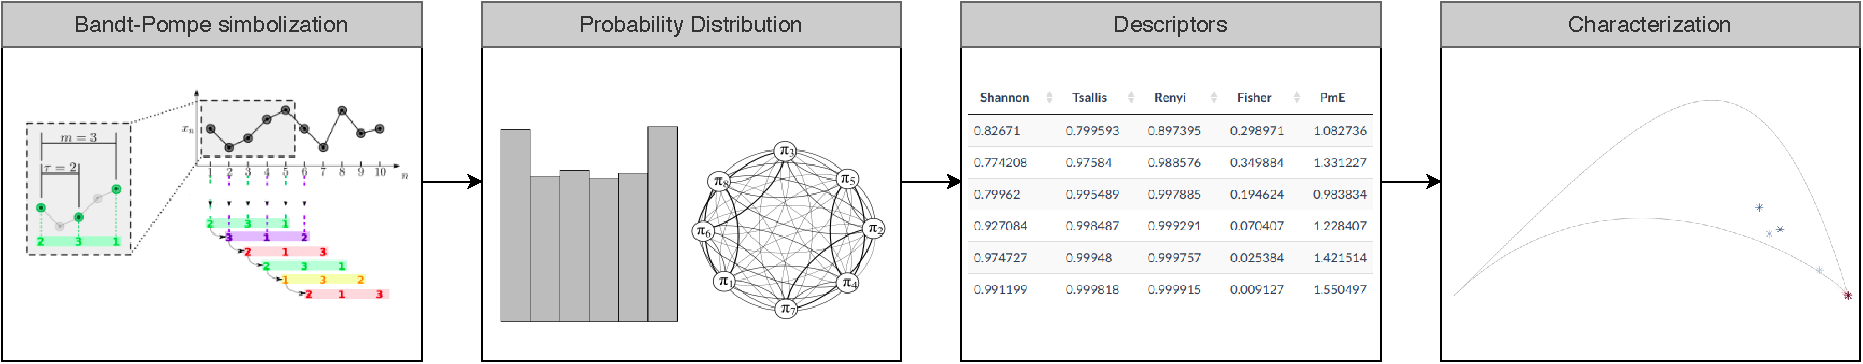
\includegraphics[width = 11cm,height = 2.6cm]{Figures/methodologyNATS.pdf}
    \end{figure}

\end{frame}

\begin{frame}{Symbolization of Bandt-Pompe}

    \begin{figure}
       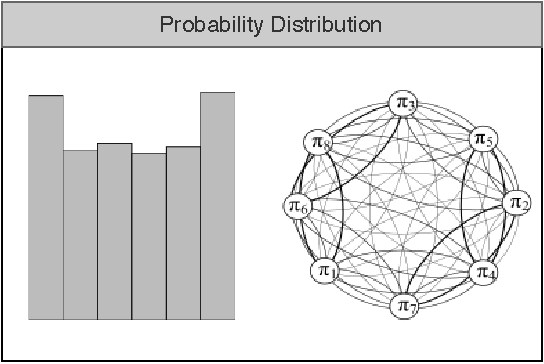
\includegraphics[scale = 0.7]{Figures/symbolization.pdf}
    \end{figure}

    \begin{itemize}
        \item Bandt-Pompe
        \item Bandt-Pompe weighted
        \item Ordinal Patterns Transition Graph
        \item Weighted Ordinal Patterns Transition Graph
    \end{itemize}

\end{frame}

\begin{frame}{Information Theory Descriptors}

    \begin{figure}
       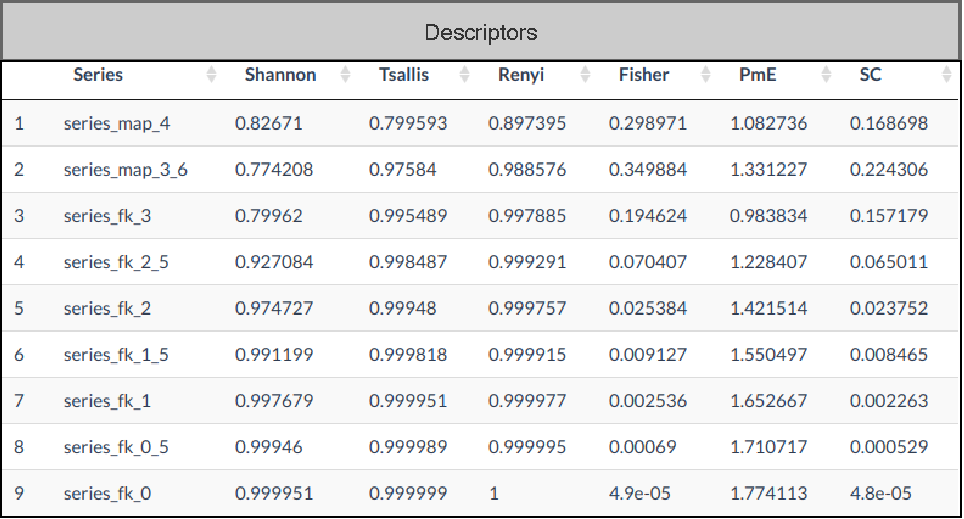
\includegraphics[scale = 0.5]{Figures/Descriptors.pdf}
    \end{figure}

    \begin{itemize}
        \item Permutation Entropy
        \item Stochastic Distances
        \item Statistical complexity
    \end{itemize}

\end{frame}


\begin{frame}{Characterization}

    \begin{figure}
      \centering
       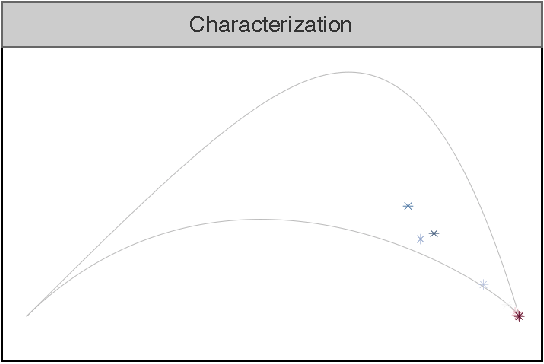
\includegraphics[scale = 0.8]{Figures/Characterization.pdf}
    \end{figure}

    \begin{itemize}
        \item HC Plane
        \item Fisher Plane
    \end{itemize}
\end{frame}

\section{Characterization of SAR image textures in the HC plane}

\begin{frame}[fragile]{Linearization Process}
    
    \vspace{2cm}

    \begin{figure}
      \centering
       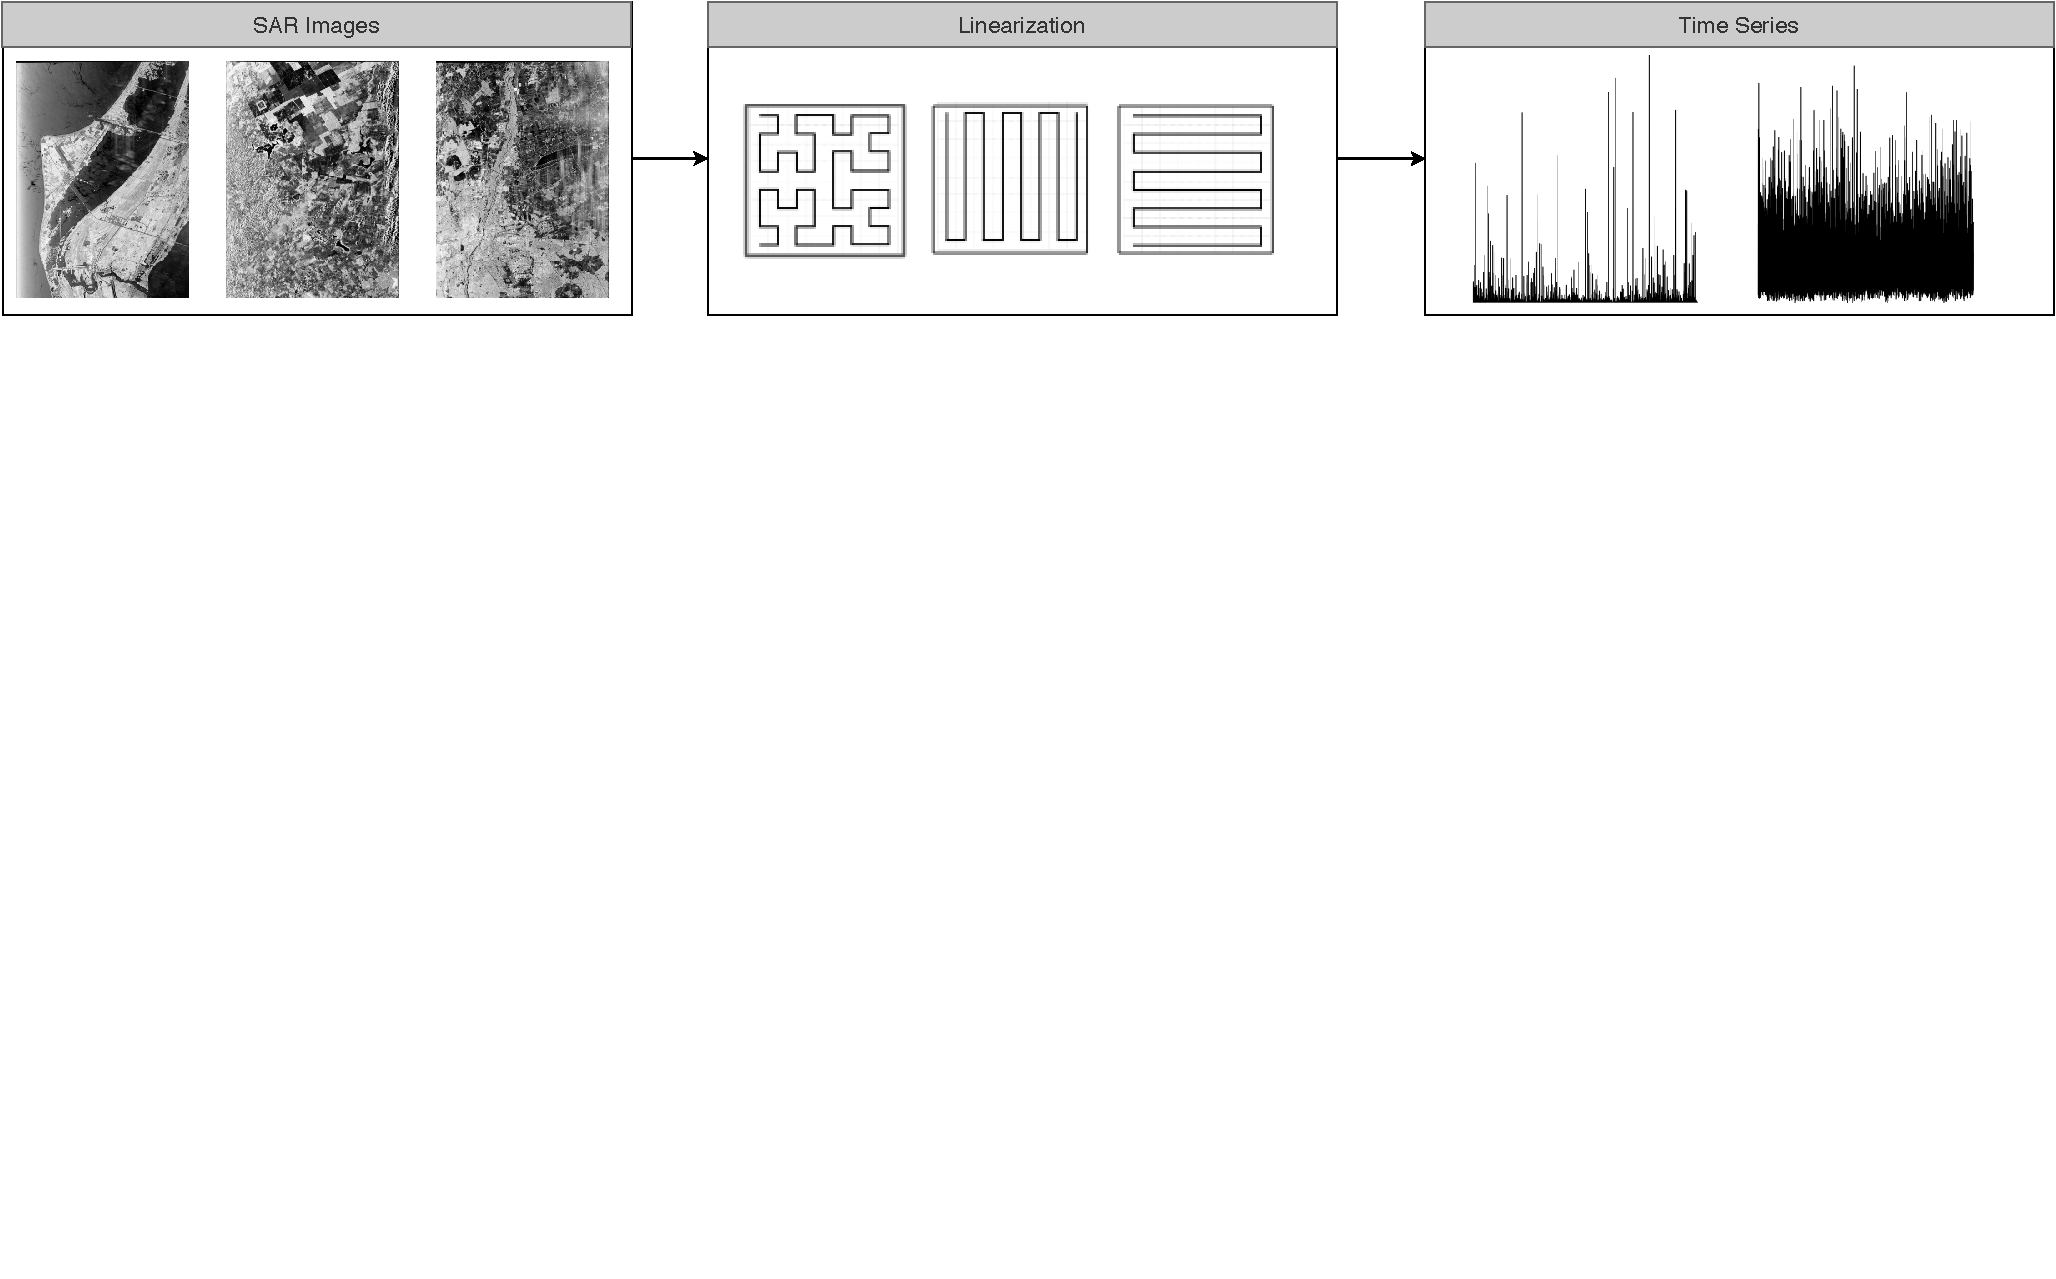
\includegraphics[width = 11cm,height = 10.6cm]{Figures/SAR.pdf}
    \end{figure}
    
\end{frame}

\begin{frame}[fragile]{Methodology}

    \begin{figure}
      \centering
       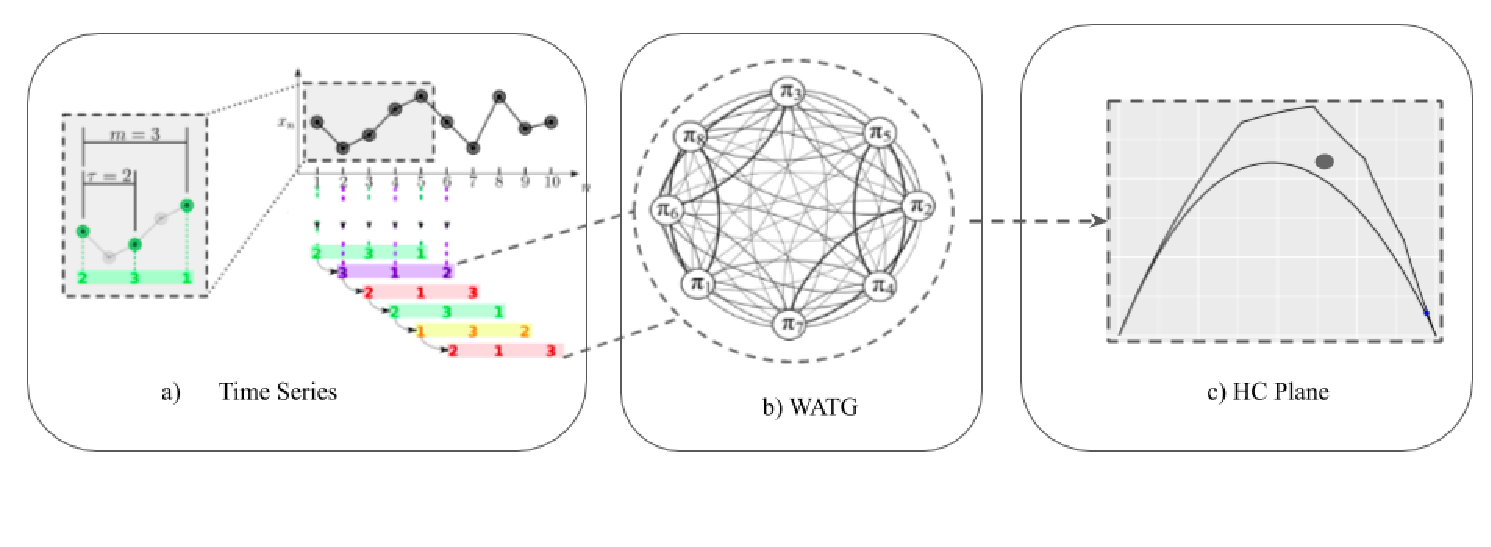
\includegraphics[scale = 0.4]{Figures/WATG.pdf}
    \end{figure}
    
\end{frame}

\maketitle

\end{document}
